\chapter{Sparse Data Operations}

The Global Arrays Toolkit contains several subroutines designed to
support operations on sparse data sets. Most sparse data objects,
such as sparse matrices, are generally described using a collection
of 1-dimensional arrays, so the operations discussed below are primarily
focused on 1D Global Arrays. The discussion of sparse data operations
will begin by describing the sparse data subroutines and then will
show how they can be used by describing an algorithm for doing a sparse
matrix-dense vector multiply.
\begin{lstlisting}[style=cppnoframe]
Fortran: subroutine ga_patch_enum(g_a, lo, hi, istart, istride)
C: void GA_Patch_enum(int g_a, int lo, int hi, int istart, int istride)
\end{lstlisting}

\noindent This subroutine enumerates the elements of an array between elements
\texttt{lo} and \texttt{hi} starting with the value istart and incrementing
each subsequent value by \texttt{istride}. This is a collective operation.
Some examples of its use are shown below:
\begin{lstlisting}[style=cpp]
    call ga_patch_enum(g_a, 1, n, 1, 1)
    g_a: 1 2 3 4 5 6 7 8 9 10 ... n
    call ga_zero(g_a)
    call ga_patch_enum(g_a, 5, n, 7, 2)
    g_a: 0 0 0 0 7 9 11 13 15 ...
    Fortran: subroutine ga_scan_copy(g_src, g_dest, g_mask, lo, hi)
    C:   void GA_Scan_copy(int g_src, int g_dest, int g_mask,int lo, int hi)
\end{lstlisting}

This subroutine does a segmented scan-copy of values in the source
array \texttt{g\_src} into a destination array \texttt{g\_dest} with
segments defined by values in an integer mask array \texttt{g\_mask}.
The scan-copy operation is only applied to the range between the \texttt{lo}
and \texttt{hi} indices. The resulting destination array will contain
segments of consecutive elements with the same value. This is a collective
operation. An example is shown below to illustrate the behavior of
this operation. 

\begin{lstlisting}[style=cppnoframe]
call ga_scan_copy(g_src, g_dest, g_mask, 1, n)
g_mask: 1 0 0 0 0 1 0 1 0 0 1 0 0 0 1 1 0
g_src: 5 8 7 3 2 6 9 7 3 4 8 2 3 6 9 10 7
g_dest: 5 5 5 5 5 6 6 7 7 7 8 8 8 8 9 10 10
Fortran subroutine ga_scan_add(g_src, g_dest, g_mask, lo, hi, excl)
C
void GA_Scan_add(int g_src, int g_dest, int g_mask, int lo, int hi, int excl)
\end{lstlisting}

\noindent This operation will add successive elements in a source vector \texttt{g\_src
}and put the results in a destination vector \texttt{g\_dest}. The
addition will restart based on the values of the integer mask vector
\texttt{g\_mask}. The scan is performed within the range defined by
the indices \texttt{lo} and \texttt{hi}. The excl flag determines
whether the sum starts with the value in the source vector corresponding
to the location of a 1 in the mask vector (\texttt{excl=0}) or whether
the first value is set equal to 0 (\texttt{excl=1}). Some examples
of this operation are given below.
\begin{lstlisting}[style=cppnoframe]
call ga_scan_add(g_src, g_dest, g_mask, 1, n, 0)
g_mask: 1 0 0 0 0 0 1 0 1 0 0 1 0 0 1 1 0
g_src: 1 2 3 4 5 6 7 8 9 10 11 12 13 14 15 16 17
g_dest: 1 3 6 10 15 21 7 15 9 19 30 12 25 39 15 16 33
call ga_scan_add(g_src, g_dest, g_mask, 1, n, 1)
g_mask: 1 0 0 0 0 0 1 0 1 0 0 1 0 0 1 1 0
g_src: 1 2 3 4 5 6 7 8 9 10 11 12 13 14 15 16 17
g_dest: 0 1 3 6 10 15 0 7 0 9 19 0 12 25 0 0 16
Fortran subroutine ga_pack(g_src, g_dest, g_sbit, lo, hi, icount)
C  void GA_Pack(int g_src, int g_dest, int g_sbit, int lo, int hi, int icount)
\end{lstlisting}

The pack routine is designed to compress the values in the source
vector\texttt{ g\_src} into a smaller destination array\texttt{ g\_dest}
based on the values in an integer mask array \texttt{g\_mask}. The
values \texttt{lo} and \texttt{hi} denote the range of elements that
should be compressed and \texttt{icount} is a variable that on output
lists the number of values placed in the compressed array. This is
a collective operation. An example of its use is shown below.
\begin{lstlisting}[style=cppnoframe]
call ga_scan_add(g_src, g_dest, g_mask, 1, n, 0)
g_mask: 1 0 0 0 0 0 1 0 1 0 0 1 0 0 1 1 0
g_src: 1 2 3 4 5 6 7 8 9 10 11 12 13 14 15 16 17
g_dest: 1 3 6 10 15 21 7 15 9 19 30 12 25 39 15 16 33
call ga_scan_add(g_src, g_dest, g_mask, 1, n, 1)
g_mask: 1 0 0 0 0 0 1 0 1 0 0 1 0 0 1 1 0
g_src: 1 2 3 4 5 6 7 8 9 10 11 12 13 14 15 16 17
g_dest: 0 1 3 6 10 15 0 7 0 9 19 0 12 25 0 0 16
Fortran subroutine ga_pack(g_src, g_dest, g_sbit, lo, hi, icount)
C  void GA_Pack(int g_src, int g_dest, int g_sbit, int lo, int hi, int icount)
\end{lstlisting}

The unpack routine is designed to expand the values in the source
vector \texttt{g\_src} into a larger destination array \texttt{g\_dest}
based on the values in an integer mask array \texttt{g\_mask}. The
values \texttt{lo} and \texttt{hi} denote the range of elements that
should be expanded and icount is a variable that on output lists the
number of values placed in the uncompressed array. This is a collective
operation. An example of its use is shown below.
\begin{lstlisting}[style=cppnoframe]
call ga_unpack(g_src, g_dest, g_mask, 1, n, icount)
g_mask: 1 0 0 0 0 1 0 1 0 0 1 0 0 0 1 0 0
g_src: 1 6 8 11 15
g_dest: 1 0 0 0 0 6 0 8 0 0 11 0 0 0 15 0 0
icount: 5
\end{lstlisting}

\section{Sparse Matrix-Vector Multiply Example}

The utility of these subroutines in actual applications is by no means
obvious so to illustrate their use, we describe a simple sparse matrix-vector
multiply. The starting point of this calculation is a compressed sparse
row (CSR) matrix in which only the non-zero elements are stored. The
CSR storage format for an NxN matrix consists of three vectors. The
first is a VALUES vector consisting of all the non-zero values contained
in the matrix, the second is a J-INDEX vector that contains all the
j indices of the values stored in the VALUES vector and the third
vector is the I-INDEX vector that contains N+1 entries and contains
the offsets in the J-INDEX vector corresponding to each row in the
matrix. The last entry in I-INDEX corresponds to the total number
of non-zero values in the sparse matrix. The VALUES and J-INDEX vectors
should contain the same number of elements. Within each row the values
are ordered by increasing values of the j index and then by increasing
values of the i index. An example of a sparse matrix and its CSR representation
is shown below. 
\begin{verbatim}
    0 0 1 3 0
    2 0 0 0 5
    0 7 0 9 0
    3 0 4 0 5
    0 2 0 0 6
\end{verbatim}
The CSR representation of this matrix is
\begin{verbatim}
VALUES: 1 3 2 5 7 9 3 4 5 2 6 

J-INDEX: 3 4 1 5 2 4 1 3 5 2 5 

I-INDEX: 1 3 5 7 10 12
\end{verbatim}
Note that each value in I-INDEX corresponds to the location of the
first element of the row in J-INDEX. The last element in I-INDEX equals
one plust the total number of non-zero elements in the matrix and
is a useful number to have available when performing sparse matrix
operations. Depending on indexing conventions, it might be more useful
to set the last element equal to the number of non-zero elements.

For a very large sparse matrix, it may be necessary to distribute
the CSR representation across multiple processors. This example assumes
that the each of the components of the CSR matrix is stored in a 1-dimensional
Global Array. To start the calculation, it is first necessary to create
the distributed CSR matrix. We assume that it is possible to assign
the evaluation of individual rows to individual processors. A simple
way of starting is to divide up the number of rows evenly between
processors and have each processor evaluate all elements of the rows
assigned to it. These can then be stored in a local CSR format. In
this case, the I-INDEX vector contains only the number of rows assigned
to the processor. In the example shown above, assume that the matrix
is divided between three processors and that processes 0 and 1 have
two rows each and process 2 has one row. The layout on the three processes
looks like
\begin{verbatim}
Process 0 

VALUES: 1 3 2 5 

J-INDEX: 3 4 1 5 

I-INDEX: 1 3 

INC: 2 2



Process 1 

VALUES: 7 9 3 4 5 

J-INDEX: 2 4 1 3 5 

I-INDEX: 1 3 

INC: 2 3



Process 2 

VALUES: 2 6 

J-INDEX: 2 5 

I-INDEX: 1 

INC: 2 
\end{verbatim}
The local array INC contains the number of non-zero elements in each
row. The total number of non-zero elements in the matrix can be found
by summing the number of non-zero values on each process. This value
can then be used to create distributed VALUES and J-INDEX arrays containing
the complete CSR matrix. A distributed I-INDEX array can be constructed
from knowledge of the original matrix dimension N. In addition to
Global Arrays representing distributed versions of VALUES, J-INDEX,
and I-INDEX, an integer Global Array of length N+1 called SBIT is
also needed. This array is initialized so that the first element is
1 and the remaining elements are all zero. To create the distributed
array I-INDEX a temporary Global Array of length N+1 is created. The
following code fragment illustrates the construction of I-INDEX

\begin{lstlisting}[style=cppnoframe]
lo = imin + 1 ! imin is lower index of i values on this processor
hi = imax + 1 ! imax is upper index of i values on this processor
if (me.eq.0) then
    call nga_put(g_tmp, one, one, one, one)
endif
call nga_put(g_tmp, lo, hi, inc, one)
call ga_sync isize = n + 1
call ga_scan_add(g_tmp,g_i_index, g_sbit, isize, 0)
\end{lstlisting}

The variable ONE is an integer variable set equal to 1. This code
fragment results in a distributed array containing the elements of
I-INDEX as described above. Note that the N+1 element in \texttt{g\_i\_index}
is equal to one plus the total number of non-zero elements. The SBIT
and TMP arrays can now be destroyed as they are no longer needed.

To execute the actual sparse matrix-vector multiply, it is necessary
to have a second bit array MASK whose length is equal to the number
of non-zero elements in the sparse matrix and which has unit values
at the locations corresponding to the start of each row in the CSR
and zeros everywhere else. This can be constructed from the I-INDEX
array in a fairly straightforward way using the \texttt{nga\_scatter
}routine. The code fragment for constructing this is
\begin{lstlisting}[style=cppnoframe]
call ga_zero(g_mask)
call nga_distribution(g_i_index, me, lo, hi)
call nga_access(g_i_index, lo, hi, idx, ld)
ntot = hi - lo + 1 
if (me.eq.ga_nnodes()-1) then
    ntot = ntot - 1
endif
do i = 1, ntot
    ones(i) = 1
end do
call nga_scatter(g_mask, ones, int_mb(idx), ntot)
call nga_release(g_i_index, lo, hi)
\end{lstlisting}

This code will create an appropriate mask array with 1\textquoteright{}s
corresponding to the start of each row in the VALUES and J-INDEX arrays.
The last element in the I-INDEX array contains the total number of
non-zero elements and does not correspond to an offset location, hence
the value of NTOT is decreased by 1 for the last processor.

Finally, the remaining task is to copy the values of the j indices
and the matrix values from the local arrays into the corresponding
Global Arrays. The code fragment for this is
\begin{lstlisting}[style=cppnoframe]
nga_get(g_i_index, imin, imin, jmin, one)
call nga_get(g_i_index, imax+1, imax+1, jmax, one)
jmax = jmax - 1
call nga_put(g_j_index, jmin, jmax, jvalues, one)
call nga_put(g_values, jmin, jmax, values, one)
\end{lstlisting}

The value of \texttt{jmax} is decreased by 1 since this represents
the start of the \texttt{imax+1} row. The value for the last row works
out correctly since we defined the N+1 element of I-INDEX to equal
one plus the total number of non-zero elements in the sparse matrix.
At this point the matrix is completely stored in a set of distributed
vectors representing a CSR storage format. An additional distributed
integer vector representing the bit mask for this matrix has also
been created.

Having created a distributed sparse matrix in CSR format, the next
step is to construct a sparse matrix-dense vector multiply. This operation
is outlined schematically in Figure~\ref{cap:SparseMatrix}. The
original sparse matrix-dense vector multiply is shown in Figure~\ref{cap:SparseMatrix}(a).
The first step, shown in Figure~\ref{cap:SparseMatrix}(b) is to
express the dense vector as a sparse matrix with the same pattern
of non-zero entries as the sparse matrix. Each row in this new matrix
represents a copy of the original vector, except that only the values
corresponding to the non-zero values of the original matrix are retained.
The third step is to multiply the two matrices together element-wise
to get a new sparse matrix with the same pattern of non-zero entries
as the original sparse matrix. This is shown in Figure~\ref{cap:SparseMatrix}(c).
The final step, shown in Figure~\ref{cap:SparseMatrix}(d), is to
sum across the rows in the product matrix to get the values of the
product vector.

%
\begin{figure}
(a)


\includegraphics[width=9cm]{sparse-a}

(b)

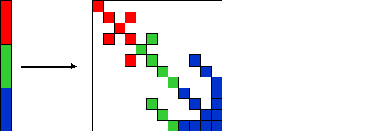
\includegraphics[width=9cm]{sparse-b}

(c)


\includegraphics[width=10cm]{sparse-c}

(d)


\includegraphics[width=9cm]{sparse-d}

\caption{\label{cap:SparseMatrix}Schematic representation of a numerical sparse
matrix-dense vector multiply.}

\end{figure}


The use of Global Array operations in implementing this operation
is described in more detail below. The original dense vector and final
product vector are assumed to be located in distributed 1D Global
Arrays with handles \texttt{g\_b} and \texttt{g\_c}, respectively.
The first step in performing the multiply operation is to create a
1D Global Array that is the same size as the original compressed matrix
VALUES array and has the same distribution across processors. Denoting
the handle of this array as \texttt{g\_tmp}, it can be filled with
the following sequence of operations
\begin{lstlisting}[style=cppnoframe]
call nga_distribution(g_j_index, me, lo, hi)
call nga_access(g_j_index, lo, hi, idx, ld)
call nga_access(g_tmp, lo, hi, id_tmp, ld)
ld = hi - lo + 1
call nga_gather(g_b, dbl_mb(id_tmp),int_mb(idx),ld)
call nga_release(g_j_index, lo, hi)
call nga_release(g_tmp,lo,hi)
\end{lstlisting}

The first three lines find the location in memory of the local portions
of the J-VALUES vector and the \texttt{g\_tmp} array. These should
both correspond to the same values of \texttt{lo} and \texttt{hi}.
The \texttt{nga\_gather} operation then copies the values of \texttt{g\_b}
in the locations pointed to by the j values represented by the index
\texttt{idx} into the corresponding locations of the local portion
of \texttt{g\_tmp}. The remaining lines release access to the local
data. Although this operation can be expressed in only a few lines
of code, it is quite complicated in terms of how it manipulates data
and may be worth spending some additional time to understand how it
works.

The element-wise multiplication of the \texttt{g\_tmp} and \texttt{g\_values}
arrays can be trivially implemented with a single call to \texttt{ga\_elem\_multiply}(\texttt{g\_tmp},
\texttt{g\_values},\texttt{ g\_tmp}). Similarly, the sum across rows
in the \texttt{g\_tmp} array can be accomplished by calling \texttt{ga\_scan\_add}(\texttt{g\_tmp},
\texttt{g\_values}, \texttt{g\_mask}, \texttt{one}, \texttt{ntot},
\texttt{0}), where \texttt{ntot} is the total number of non-zero elements.
At this point the values of the product vector are located at the
elements just before the locations indicated by the g\_mask array.
To get these values back into an ordinary compressed vector, the g\_mask
vector is shifted to the left by one place, using the following code
fragment
\begin{lstlisting}[style=cppnoframe]
call nga_distribution (g_mask, me, lo, hi)
call nga_access(g_mask, lo, hi, idx, ld)
ld = hi-lo
isav = int_mb(idx)
do i = 1, ld
    int_mb(idx + i - 1) = int_mb(idx + i)
end do
if (lo.eq.1) then
    ldx = isize
else
    idx = lo-1
endif 
call nga_release(g_mask, lo, hi)
call ga_sync
call nga_put(g_mask, idx, idx, isav, ld)
call g_sync
\end{lstlisting}

The results in \texttt{g\_tmp} can now be packed into the final results
vector \texttt{g\_c} using a single call to \texttt{ga\_pack}(\texttt{t\_tmp},
\texttt{g\_c}, \texttt{g\_mask}, \texttt{one}, \texttt{ntot}, \texttt{icnt}). 
